\documentclass{article}
\usepackage{main}

\title{Extremums d'une fonction}
\date{25 Mars 2024}
\author{Seconde 9}

\begin{document}
\maketitle
\section{Course de dauphins}
Deux dauphins, Flora et Gaétan, font un concours de sauts de catégorie \og \qty{20}{\m} \fg : Ils nagent en ligne droite sur une distance de \qty{20}{\m}, et le vainqueur est celui qui saute le plus haut au terme de cette distance. On note $f(x)$ (respectivement $g(x)$) l'altitude en mètres de Flora (respectivement Gaétan) en fonction de la distance $x$ parcourue. Les courbes représentatives $\mathcal{C}_f$ et $\mathcal{C}_g$ sont données ci-après.
\begin{center}
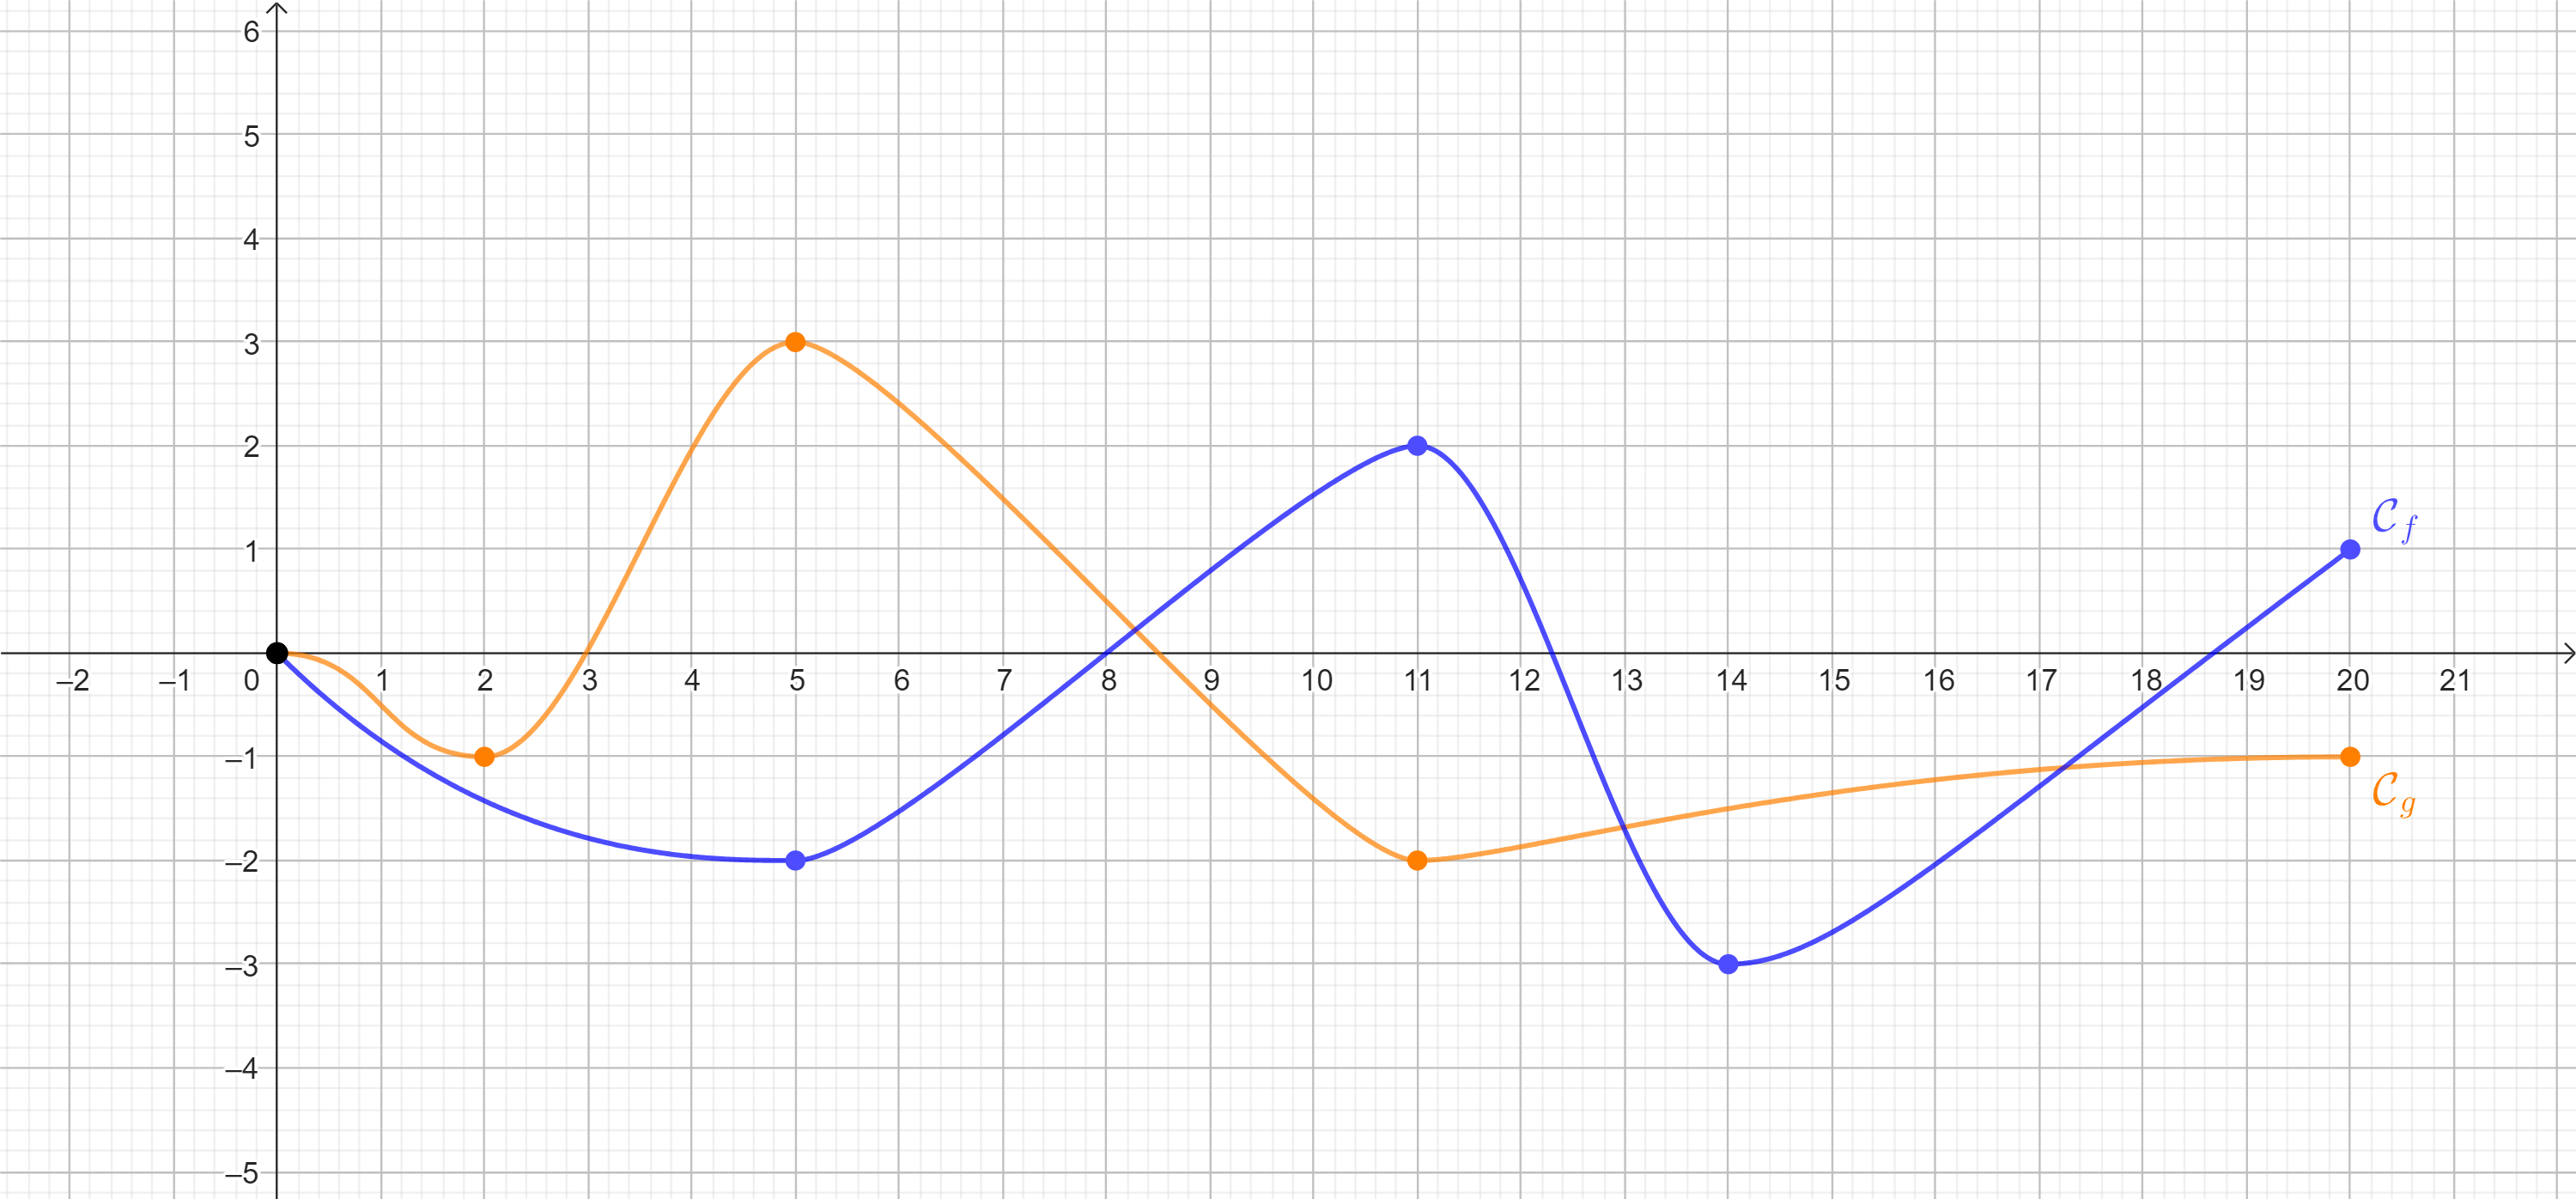
\includegraphics[scale=0.7]{Graphique.png}
\end{center}
\begin{enumerate}
\item À quoi correspond une altitude négative durant cette compétition ?
\item Déterminer la hauteur du plus haut saut de Flora.
\item Qui est le vainqueur du concours ? Justifier.
\item Qui serait le vainqueur si ce concours était un concours de plongée ? Justifier.
\end{enumerate}
\newpage
\section{Deuxième course}
Nous n'avons pas pu assister au concours opposant Ada et Bob. Heureusement, un spectateur nous rapporte les points culminants de chacun des participants à l'aide d'un tableau de variations. Les fonctions correspondant aux altitudes d'Ada et Bob sont données par $a$ et $b$.
\begin{center}
\begin{tikzpicture}[scale=0.8]
\tkzTabInit{$x$ /0.5, $a(x)$/2, $b(x)$/2}{$0$, $5$, $10$, $15$, $20$, $25$, $30$};
\tkzTabVar{+/$0$,-/$-2$,R/,+/$3$,-/$-1$,+/$1$,-/$0$};
\tkzTabVar{+/$0$,-/$-1$,+/$2$,R/,-/$-3$,R/,+/$2$};
\end{tikzpicture}
\end{center}
\begin{enumerate}[resume*]
\item Quelle est la catégorie de la compétition entre Ada et Bob ?
\item Qui est le vainqueur de la compétition de saut ?
\item Si la compétition était de catégorie \og \qty{15}{\m} \fg, a-t-on assez d'informations pour déterminer le vainqueur ?
\item Tracer sur le repère suivant deux courbes représentatives possibles pour les fonctions $a$ et $b$. D'après votre représentation, qui serait le vainqueur de la catégorie \og \qty{15}{\m} \fg 
\end{enumerate}
\begin{center}
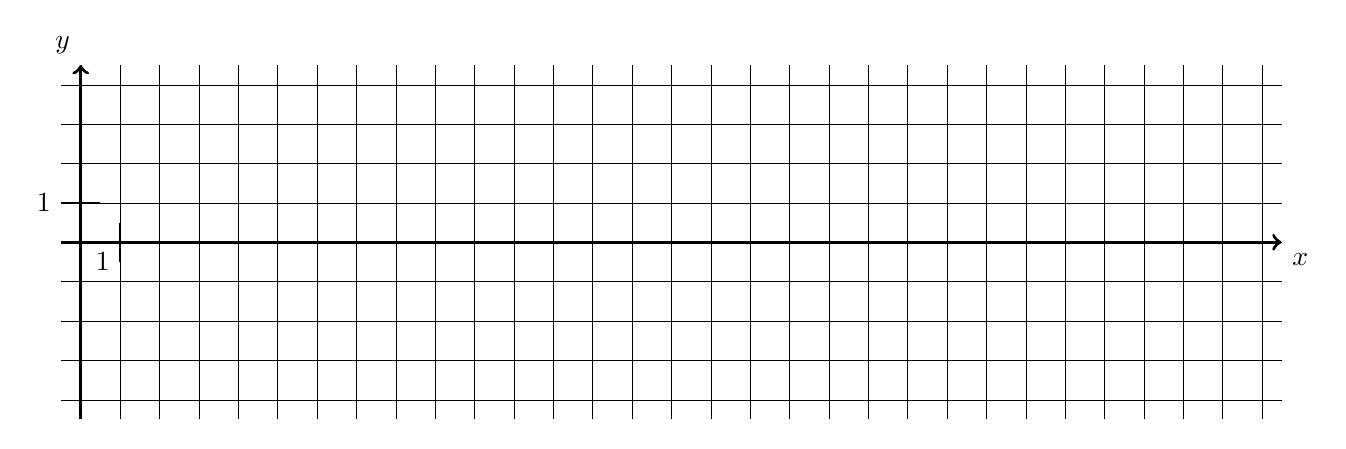
\begin{tikzpicture}
\draw[ultra thin] (-0.25,-2.25) grid[step=0.5] (15.25,2.25);
\draw[->,very thick] (0,-2.25) -- (0,2.25) node[above left] {$y$};
\draw[->,very thick] (-0.25,0) -- (15.25,0) node[below right] {$x$};
\draw[thick] (0.5,0.25) -- (0.5,-0.25) node[left] {$1$};
\draw[thick] (0.25,0.5) -- (-0.25,0.5) node[left] {$1$};
\end{tikzpicture}
\end{center}
\end{document}